
%(BEGIN_QUESTION)
% Copyright 2014, Tony R. Kuphaldt, released under the Creative Commons Attribution License (v 1.0)
% This means you may do almost anything with this work of mine, so long as you give me proper credit

Calculate all listed values for this transformer circuit:

$$\includegraphics[width=15.5cm]{i01256x01.eps}$$

\begin{itemize}
\item{} $V_{primary} = $
\item{} $V_{secondary} = $
\item{} $I_{primary} = $
\item{} $I_{secondary} = $
\end{itemize}

Explain whether this is a {\it step-up}, {\it step-down}, or {\it isolation} transformer, and also explain what distinguishes the ``primary'' winding from the ``secondary'' winding in any transformer.

\underbar{file i01256}
%(END_QUESTION)





%(BEGIN_ANSWER)

\begin{itemize}
\item{} $V_{primary} = 48 \hbox{ volts}$
\item{} $V_{secondary} = 14.77 \hbox{ volts}$
\item{} $I_{primary} = 30.3 \hbox{ mA}$
\item{} $I_{secondary} = 98.5 \hbox{ mA}$
\end{itemize}

This is a {\it step-down} transformer.

%(END_ANSWER)





%(BEGIN_NOTES)

Most transformer problems are nothing more than ratios, but some students find ratios difficult to handle.  Questions such as this are great for having students come up to the board in the front of the classroom and demonstrating how they obtained the results.

%INDEX% Electronics review: transformer ratios

%(END_NOTES)


